\title{A 90 Minute \textit{SAGA} Hands-On Tutorial\\[1em]
\Large{ISSGC, Nice, France, July 5-17 2009 } \\[1em]
\large{Ole Weidner, Hartmut Kaiser, Andre Merzky, Shantenu Jha}}

\documentclass[12pt]{article}

 \usepackage{graphicx}

\usepackage{color}
\newif\ifdraft
\drafttrue
\ifdraft
\newcommand{\amnote}[1]{   {\textcolor{magenta} { ***Andre: #1 }}}
\newcommand{\olenote}[1]{{\textcolor{blue}    { ***Ole: #1 }}}
\newcommand{\hartmutnote}[1]{  {\textcolor{green}     { ***Hartmut:    #1 }}}
\newcommand{\jhanote}[1]{  {\textcolor{red}     { ***Shantenu:    #1 }}}
 \usepackage[pdftex,colorlinks=true, linkcolor=blue,citecolor=blue,
       urlcolor=blue]{hyperref}
\else
\newcommand{\amnote}[1]{}
 \newcommand{\olenote}[1]{}
\newcommand{\note}[1]{}
\newcommand{\hartmutnote}[1]{}
 \newcommand{\jhanote}[1]{}
\fi
\begin{document}

\maketitle

%\begin{abstract}
%This is the paper's abstract \ldots
%t\end{abstract}

\section*{Scope of this Tutorial}
The scope of this tutorial is to provide the audience with the required resources and technical knowledge (hands-on experience) to start hacking their own distributed applications with SAGA.

\subsection*{Prerequisites} This tutorial requires basic knowledge of the C/C++ programming language. Experience using the command line on a Linux/UNIX based operating system and a basic idea of what a compiler, a linker and a Makefile is might come in handy.\\[0.4em]
Unless this tutorial is going to be preceded by a SAGA installation tutorial, the students are required to have a fully working installation of SAGA on their laptops/lab machines (preferred), or remote access (e.g. via SSH) to a machine with SAGA installed. 
	
%\subsection*{Cheat Sheat} At the beginning of the tutorial we're going to hand out the SAGA Cheat Sheet (yet to be %created). The cheat sheet is a double-sided % (laminated, so people won't throw it away!)
%letter-sized piece of paper with hints and tips for writing, compiling, and running SAGA applications.

\subsection*{ISSGC Infrastructure}

\begin{figure}[!ht]
  \begin{center}
      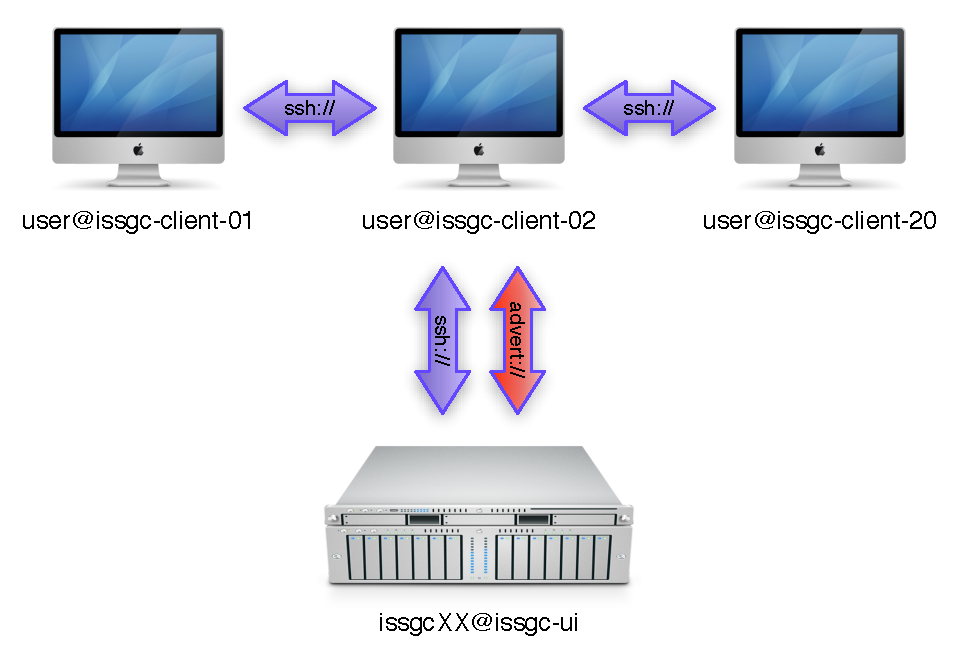
\includegraphics[width=1\textwidth]{infrastructure}
 \end{center}
\end{figure}


The summer school infrastructure consists of a set of client machines issgc-client-01 to issgc-client-20 and a server issgc-ui. Since SAGA provides a uniform API for job submission, it doesn't make a difference to the wether you submit your jobs through gLite, Globus, Condor or any other middleware. For the sake of simplicity, we set up the machines with SSH in a way that allows you to submit "jobs" to any other client or the server and transfer data between all available machines. Before you start using SAGA, please make sure that SSH work on your lab machine:

\begin{verbatim}
ssh user@issgc-client-XX /bin/hostname
ssh issgcXX@issgc-ui /bin/hostname
\end{verbatim}

Remember these host names. You will use them again in your SAGA program in the form of:

\begin{verbatim}
saga::url my_resource("ssh://user@issgc-client-XX");
saga::url my_other_resource("ssh://issgcXX@issgc-ui");
\end{verbatim}

The server also hosts a SAGA advert DB (PostgreSQL). You will use it in one of the exercises to
store some data. To make sure that you don't mess with each other's data, we created directories
for each participant - make sure that you can access yours:

\begin{verbatim}
source /opt/saga-1.3.1-issgc/share/saga/saga-env.sh
saga-advert list_directory advert://issgc-ui//issgcXX/ ?
\end{verbatim}




\subsection*{Unit I (15 min)} \textbf{A minimal SAGA application.} Every application that uses just a single SAGA call is considered a SAGA applications, since it triggers the whole stack. SAGA is not a framework. It doesn�t impose a specific programming model or way to use it  (like, e.g. MPI). Look at it as a TOOLBOX for distributed computing.

\jhanote{Remember, we are going to use SSH adaptors for everything and nothing will USE Globus}

\jhanote{Points/Issues to consider here: (i) Avoid Context, (ii) Copy a file given 2 URLS, and (iii) Command line Tools. Make Use of material already in the programming manual}

\begin{verbatim}

\end{verbatim}

\subsection*{Unit II (15 min)} \textbf{Compiling and linking.} Demonstrate how to include the SAGA Makefiles to compile and link a SAGA application. Explain the concept of packages as independent shared libraries. Demonstrate static vs. dynamic linking.

\begin{verbatim}
<CODE>
\end{verbatim}

\subsection*{Unit III (15 min)} \textbf{Running a SAGA application.}
Explain what needs to be in the loader path. Explain the effects of SAGA\_VERBOSE and how it can be used to debug a saga application. Demonstrate how the engine launches adaptor loading, etc... in the background.

\begin{verbatim}
<CODE>
\end{verbatim}

\section*{Unit IV (20 min)}\textbf{SAGA-based Applications:}
In this tutorial, we will work with three different examples. The aim of these
applications is to give you a  quick feel for how SAGA is actually utilized to develop distributed applications. And although these examples are by definition very simple, they are representative of the way you would use SAGA in a real world examples to develop many of the scientific applications you heard about in today's 
lecture such as Replica-Exchange and C0$_2$ Sequestration problem(s).

In the first example, we will introduce a simple ``Hello Distributed World!'', where the aim will be to submit three simple remote jobs using SAGA. In the second example application (``chaining\_jobs.cpp''), we will serialize the launch of three (remote) jobs, so that the second job is launched after the first, and the third job is launched after the second. In the third example application (``depending\_jobs.cpp''), we will start an application that once started, is able to re-spawn itself on another machine and after doing so increments a ``global counter''. Finally, we will leave you with a programming excercise that will build upon your understanding of application examples 2 and 3.

\subsection*{Example 1: Hello distributed world!} Submit three jobs to three machines. One returns �Hello�, one returns �Distributed� and one returns �World�. They may or may not return in the right order. This should give the student an idea how they could potentially speed up their application using multiple resources. 


\begin{verbatim}
// The hello_world example is meant to be a very simple and first example to 
// try when it comes to SAGA. It's purpose is to spawn 3 (possibly remote) 
// identical jobs (/bin/echo) while passing the 3 words "Hello", "distributed", 
// and "world!" on their command lines. The result is that the jobs will print
// the respective command line arguments (hey, it's /bin/echo we're 
// launching...). The master job (this one) waits for the 3 child jobs to 
// finish. It intercepts the generated output and prints it to the user.
//
// Depending on which child jobs finish first the overall printed message might
// be some combination of the 3 arguments we passed. But most of the time you
// will see "Hello distributed world!", which is our way of saying hello and
// welcome to the world of SAGA.


// the routine spawning the SAGA jobs and waiting for their results
void run_a_job(std::string host, std::string argument)
{
    try {
        saga::job::service js (host);
        saga::job::ostream in;
        saga::job::istream out;
        saga::job::istream err;

        // run the job
        saga::job::job j = js.run_job("/bin/echo " + argument, host, in, out, err);

        // wait for the job to finish
        saga::job::state s = j.get_state();
        while (s != saga::job::Done && s != saga::job::Failed)
            s = j.get_state();

        // if the job finished successfully, print the generated output
        if (s == saga::job::Done) {
            std::string line;
            while (!std::getline(out, line).eof())
                std::cout << line << '\n';
        }
        else {
            std::cerr << "SAGA job: " << j.get_job_id() << " failed (state: " 
                      << saga::job::detail::get_state_name(s) << ")\n";
        }
    }

   catch (saga::exception const& e) {
        std::cerr << "saga::exception caught: " << e.what () << std::endl;
    }
    catch (std::exception const& e) {
        std::cerr << "std::exception caught: " << e.what () << std::endl;
    }
    catch (...) {
        std::cerr << "unexpected exception caught" << std::endl;
    }
}

///////////////////////////////////////////////////////////////////////////////
int main(int argc, char* argv[])
{
    // run 3 separate threads executing the saga calls
    boost::thread t1 (run_a_job, HOST1, "Hello");
    boost::thread t2 (run_a_job, HOST2, "distributed");
    boost::thread t3 (run_a_job, HOST3, "world!");

    // wait for all spawned threads to finish
    t1.join();
    t2.join();
    t3.join();
    return 0;
}

\end{verbatim}

\subsection*{Example 2: Multiple Sequential Jobs} \textbf{Applications} The aim of this section is to see how SAGA is used to implement common {\it higher-level} functionality that is used by Distributed Applications (DA). Specifically, we will look at two commonly occuring functionality required by DA.

{\bf Example 1:} Here we will demonstrate the ability to checkpoint, use a specified resource, self-migrate and restart on a different computational resource. There are multiple reasons this might be required (see lecture notes). Here we will demonstrate this capability using the \textbf{Hello distributed world!} example discussed in Unit IV.  Instead of launching three jobs on three machines, we will launch one job on one machine, which will then launch itself on another machine, which in turn will do so onto yet another machine. 

\begin{verbatim}
//////////////////////////////////////////////////////////////////////////////
// The chaining_jobs example tries to overcome one of the limitations of the 
// hello_world example: it introduces dependencies between 3 (possibly remotely)
// spawned childs. In this example the next child will be spawned only after 
// the previous one has finished its execution. To make it more interesting we 
// now use /usr/bin/bc to do some calculations, where the result of the previous
// calculation is used as the input for the next one.
//
// Try to make more complex calculations if you like!
///////////////////////////////////////////////////////////////////////////////

///////////////////////////////////////////////////////////////////////////////
// the routine spawning the SAGA jobs and waiting for their results
std::string increment(std::string host, std::string argument)
{
    try {
        saga::job::service js (host);
        saga::job::ostream in;
        saga::job::istream out;
        saga::job::istream err;

        // run the job
        saga::job::job j = js.run_job("/usr/bin/bc -q", host, in, out, err);

        // wait for the job to finish
        saga::job::state s = j.get_state();
        while (s != saga::job::Running && s != saga::job::Failed)
            s = j.get_state();

        // if the job didn't start successfully, print error message
        if (s == saga::job::Failed) {
            std::cerr << "SAGA job: " << j.get_job_id() << " failed (state: " 
                      << saga::job::detail::get_state_name(s) << ")\n";
            return argument;
        }

        // feed the remote process some input
        in << "1 + " + argument + "\n";

        // receive result
        std::string line;
        std::getline(out, line);

        // quit remote process
        in << "quit\n";

        return line;
    }
    catch (saga::exception const& e) {
        std::cerr << "saga::exception caught: " << e.what () << std::endl;
    }
    catch (std::exception const& e) {
        std::cerr << "std::exception caught: " << e.what () << std::endl;
    }
    catch (...) {
        std::cerr << "unexpected exception caught" << std::endl;
    }
    return argument;    // by default just return argument
}

///////////////////////////////////////////////////////////////////////////////
int main(int argc, char* argv[])
{
    // run 3 separate threads executing the saga calls
    std::string result = increment(HOST1, "1");
    result = increment(HOST2, result);
    result = increment(HOST3, result);

    std::cout << "The overall result is: " << result << std::endl;

    return 0;
}

\end{verbatim}

Once developed, this capability can be utilized by a wide range of different applications. In other words this capability described/shown above is independent of any specific application logic. Do you know of a (Scientific) application that could utilize this feature?

\subsection*{Example 3: Managing Dependies between Jobs}

{\bf An additional Real World Example} Here we will briefly discuss MapReduce -- a computational pattern made famous by Google's use for its Search Engine Infrastructure.  The fundamental idea is that there is a Master which coordinates the distribution of work to a large number of Workers, and manages the merging of the output of the computation that the Workers produce. In addition to performance, a fundamental challenge is the need to be able to coordinate Master-Workers across a wide range of distributed systems.

\begin{verbatim}
<CODE>
\end{verbatim}

Not surprisingly the code snippet above is independent of any application specific details and focusses on the assignment of workloads to workers, execution and then retrival. This specific approach adopted here relies heavily on the use of the Advert Service.  Although introduced in the context of MapReduce, the requirement of coordination of distributed, often heteregenous units is a fundamental {\it vector} of distributed applications. (See Lecture Notes).


\subsection*{Programming Excercise:} Have the students write a distributed application We have to come up with something neat, fun!!!, and simple enough that can be solved by all students within 20 minutes and the help of the cheat sheet. 

\begin{verbatim}
<CODE>
\end{verbatim}

\subsection*{Conclusion}

\end{document}
